
\chapter{Data Visualisation}
\section{Definition}.
Data visualization is the graphical representation of information and data. By using visual elements like charts, graphs, and maps, data visualization tools provide an accessible way to see and understand trends, outliers, and patterns in data.\\

In the world of Big Data, data visualization tools and technologies are essential to analyze massive amounts of information and make data-driven decisions
THE DEADLY IMPACT of COVID-19 is driving a massive amount of research that aims at understanding the various characteristics of the pandemic. While there is no vaccine, considerable effort has been devoted to understanding the spread of the disease in different places in the world. The speed with which the disease has spread throughout the world demands agile solutions to understand and estimate the disease progression.\\

Interactive dashboards with several charts surfaced in different formats to offer concise ways to express the pandemic’s growth. Figure 1.1 illustrates some examples. The dashboard developed by Johns Hopkins University (JHU)1 was the first to track and display information on cases and death totals for different countries and states in the United States.\\

Along with lists of total counts and histograms, a bubble map composed of circles of different radii allows a visual inspection of how serious the pandemic is around the world.\\

Interesting plots were created on news outlets such as the New York Times (NYT)2,3 and the Washington Post.3 For example, NYT used Choropleth maps, a representation where geographical regions (countries or states) are mapped to colors associated with a measurement for that region (e.g., number of cases).\\

This representation is useful to communicate trends, such as the average daily counts for the past week. Similarly, they display the time series evolution for each region using line heatmaps, where daily values are mapped to colors and displayed in a row.\\

Our work (described in more detail in the following) used both Choropleth maps and line heatmaps in the development of dashboard specially designed for Brazil. Using a focus-pluscontext interface with coordinated views, the user can inspect the context using two Choropleth maps (one for the states and a second for a state selected), as well as details using two matrix heatmaps (collection of stacked line heatmaps) for states and cities. The tool displays daily or cumulative data, absolute or relative to population, and supports filtering by a time interval.\\

A vast collection of community-developed dashboards and interactive tools about COVID19 are available. Good starting places to look are the data hub hosted by Tableau and the top 100 R-resources organized by Soetewey.4 In-depth analysis is available at sites, such as Our World in Data, 5 Bing, 6 and the COVID Tracking Project, 7 among others. After developing the Brazilian dashboard, we devoted our efforts to create a set of tools to compare the spread of COVID-19 data in different regions of the world.8 We collected data from more than 6 000 locations in the world, and our interface has different charts that support visualizing multiple locations in a single chart.\\

Since the pandemic is at different stages in the world, we allow the user to align the time-series of data by a certain data the series passes a given threshold (e.g., after 100 cases). This representation is useful to observe when different locations passed through specific checkpoints (top of Figure 2).\\

While our initial charts support the comparison of different regions, the tool required the user to drive the process of choosing the regions to compare.\\

From the beginning, we felt the need to have an automatic tool that could, given a region of interest, return the closest regions given a similarity function. Looking at the disease’s spread in distinct places, but with similar growth patterns, can be useful to predict behaviors.\\

Thus, we developed a search engine to support queries using different similarity functions. For example, at the bottom of Figure 2, we show the results of searching for regions similar to Italy concerning the number of deaths.\\

The results are listed in a ranking, with pairwise comparisons that detail attributes of the different locations and evolution charts, aligned by the day of the first death. We observe the similarities in the evolution in the number of deaths and cases for Italy, France, Spain, and the United Kingdom.\\

While using the tool, we also saw similarities among cities from Brazil and the United States, both countries with large COVID-19 numbers.\\

The examples so far give a glimpse of how data visualization can help in the understanding of COVID-19. Figure 3 illustrates other applications where data visualization can help. The first example shows how multidimensional projections and network visualizations can help the literature exploration of papers that describe novel coronavirus research.\\

As new research about COVID-19 is published, there is a great need to review up-to-date literature and treatments conveniently.\\

Contact tracing is another application that relies on graph visualization to trace the network of people who may have been in contact with a COVID-19 patient, an activity essential to control the dissemination of the disease and essential for directing social distancing regulations. Graph visualization is also important in for social media spread and fact checking. \\

With many people at home, social networks are playing a significant role in people’s lives these days. Unfortunately,.\\

the dissemination of fake news and automated posting from robots is also rising. Fact-checking over the propagation network can help identify misleading information and patterns of dissemination.\\

The fourth and final example highlights the importance of data visualization in the analysis of scientific simulations.\\

It shows the visualization of simulating the transport and spread of novel coronavirus in closed spaces,9 which shows how an infected person can disseminate the virus indoors.\\

Many other examples include data visualization in the analysis of COVID-19 data, and many more is surfacing every day. We hope this summary highlights interesting examples, give pointers to other references, and motivate people to pursue other applications. 
\section{The advantages and benefits of good data \\ visualization}
Our eyes are drawn to colors and patterns. We can quickly identify red from blue, square from circle. Our culture is visual, including everything from art and advertisements to TV and movies.\\

Data visualization\cite{dataviz} is another form of visual art that grabs our interest and keeps our eyes on the message. When we see a chart, we quickly see trends and outliers. If we can see something, we internalize it quickly. It’s storytelling with a purpose. If you’ve ever stared at a massive spreadsheet of data and couldn’t see a trend, you know how much more effective a visualization can be.\\

As the “age of Big Data” kicks into high-gear, visualization is an increasingly key tool to make sense of the trillions of rows of data generated every day. Data visualization helps to tell stories by curating data into a form easier to understand, highlighting the trends and outliers. A good visualization tells a story, removing the noise from data and highlighting the useful information.\\

However, it’s not simply as easy as just dressing up a graph to make it look better or slapping on the “info” part of an infographic. Effective data visualization is a delicate balancing act between form and function. The plainest graph could be too boring to catch any notice or it make tell a powerful point; the most stunning visualization could utterly fail at conveying the right message or it could speak volumes. The data and the visuals need to work together, and there’s an art to combining great analysis with great storytelling.


\section{Why data visualization is important for any career}
It’s hard to think of a professional industry that doesn’t benefit from making data more understandable. Every STEM field benefits from understanding data—and so do fields in government, finance, marketing, history, consumer goods, service industries, education, sports, and so on.
While we’ll always wax poetically about data visualization (you’re on the Tableau website, after all) there are practical, real-life applications that are undeniable. And, since visualization is so prolific, it’s also one of the most useful professional skills to develop. The better you can convey your points visually, whether in a dashboard or a slide deck, the better you can leverage that information.
The concept of the citizen data scientist is on the rise. Skill sets are changing to accommodate a data-driven world. It is increasingly valuable for professionals to be able to use data to make decisions and use visuals to tell stories of when data informs the who, what, when, where, and how. While traditional education typically draws a distinct line between creative storytelling and technical analysis, the modern professional world also values those who can cross between the two: data visualization sits right in the middle of analysis and visual storytelling.
\section{The different types of visualizations}
When you think of data visualization, your first thought probably immediately goes to simple bar graphs or pie charts. While these may be an integral part of visualizing data and a common baseline for many data graphics, the right visualization must be paired with the right set of information. Simple graphs are only the tip of the iceberg. There’s a whole selection of visualization methods to present data in effective and interesting ways.\\

\textbf{Common general types of data visualization:}
\begin{itemize}
\item Charts;
\item Tables;
\item Graph.
\item Maps.
\item Infografics.
\item Dashboards.
\end{itemize}

\begin{figure}[htbp]
\centerline{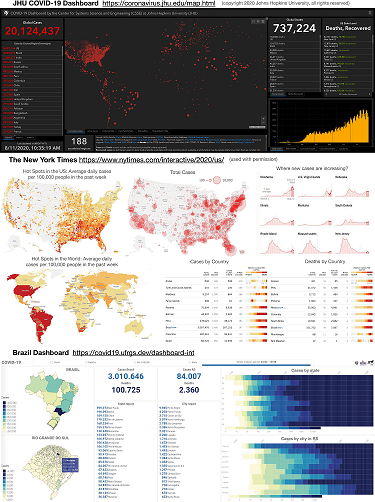
\includegraphics{Chapitre1/dashboard.png}}
\caption{Examples of data visualization in action.}
\label{fig}
\end{figure}